\chapter{Literature review}
\section{General Introduction to Ferromagnetics}

\subsection{Origin of Ferromagnetism}
In all materials electrical, chemical and magnetic properties are determined by the electronic structure. Electrons are distributed in specific shells at definite distances from the nucleus, which is due to the different energy level in each shell. In the FM elements, including $\alpha$-Fe, Co, Ni and Gd, there are three important features:

\begin{enumerate}
\item There must be an unfilled inner electron shell within the atom.
\item There must be uncompensated electronic spins in the unfilled inner shell.
\item The atoms must form a crystal lattice having a lattice constant at least 3
times the radius of the unfilled electron shell.
\end{enumerate}

Electrons have an intrinsic property called spin that contributes to their magnetic moment. The classical model of electron spin is the electron spinning on its
axis, i.e. either spin-up or spin-down. Macroscopic magnetic properties of materials are a consequence of magnetic moments associated with individual electrons, which is the sum of spin moment Figure~\ref{fig:electron}a and orbital moment Figure~\ref{fig:electron}b.

The magnetic susceptibility $\chi$ is a dimensionless proportionality
constant that indicates the degree of magnetization of a material in response to an applied magnetic field, and is given by:
\begin{equation}
\chi = \frac{M}{H}
\end{equation}
where $\chi$ is the magnetic susceptibility, $M$ is the magnetization of the material, and $H$ is the applied field.

\begin{figure}[H]
\centering
\captionsetup{justification=centering,margin=2cm}
	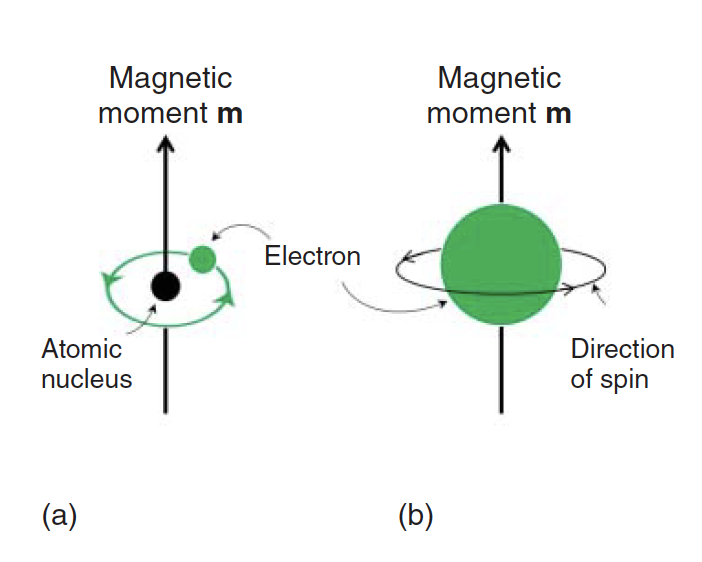
\includegraphics[height=70mm]{fig/review/electron.png}
	\caption[Diagram showing the magnetic moment associated with orbital and spin motion of an electron.]{Diagram showing the magnetic moment associated with (a) orbital motion and (b)spin motion of an electron.}
\label{fig:electron}
\end{figure}

Depending on the magnetic ordering and the sign, magnitude and
temperature dependence of the magnetic susceptibility, the magnetic materials are classified into diamagnetic, paramagnetic (PM), ferromagnetic (FM), antiferromagnetic (AFM) and ferrimagnetic (FiM) materials.

\subsection{Types of magnetism}\label{sec:ordering}
As it was stated in terms of magnetization, materials can be classified into diamagnetic, PM, FiM,  FM and AFM as it is shown in Figure \ref{fig:magneticorder}.

\begin{figure}[H]
	\centering
	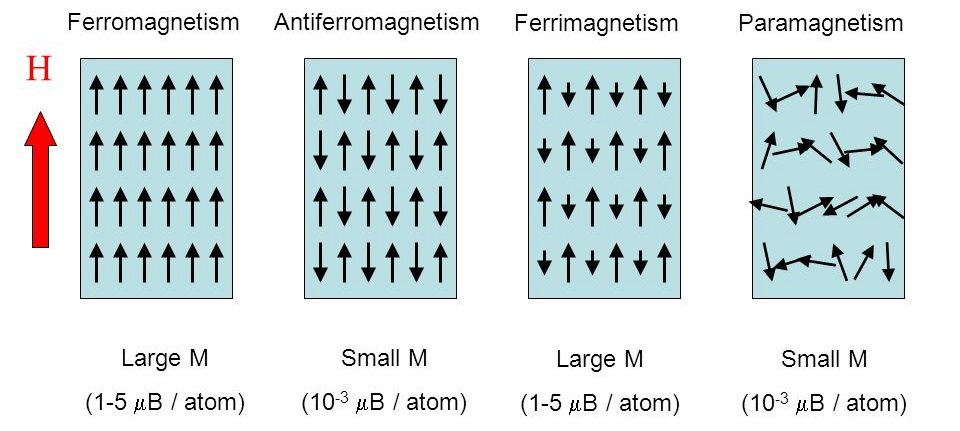
\includegraphics[width=130mm]{fig/review/magneticorder.png}
	\caption[Schematic illustration of various types of magnetism.]{Schematic illustration of various types of magnetism.}
\label{fig:magneticorder}
\end{figure}

A FM material usually forms permanent magnet or is attracted to magnets, and it undergoes phase change to PM above Curie temperature $(T_C)$ through a second-order phase transition.
FM (including FiM) is the strongest type; it is the only type that creates forces strong enough to be felt and is responsible for the common phenomena of magnetism encountered in everyday life.
An AFM has magnetization microscopically but has no macroscopic magnetization due to the cancelation of antiparallel spins of alternative layers. 
The temperature from an AFM to PM phase transition is called Néel temperature. FiM is a relatively weak FM, such as \ce{CoFe_2O_4} spinel. A diamagnetic generates weak but negative magnetization when a magnetic field is applied. 

Figure \ref{fig:table2} houses characteristic types of magnetization of pure elements in a solid-state and low temperature.

\begin{figure}[H]
	\centering
	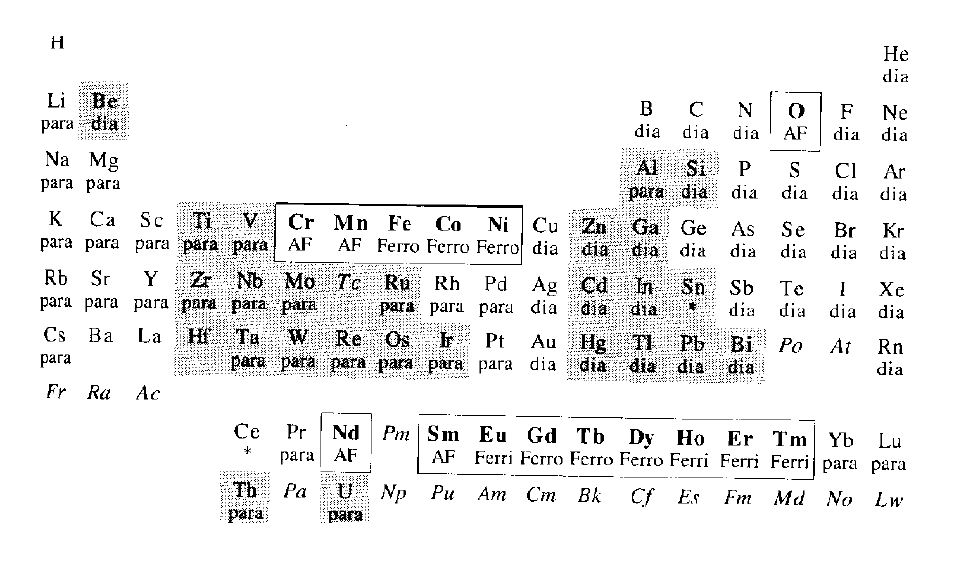
\includegraphics[width=100mm]{fig/review/tabel2.png}
	\caption[Magnetic properties of pure elements]{The magnetic properties of pure elements in a solid state at low temperature.}
	\label{fig:table2}
\end{figure}


A magnetic solid, made up of atoms with magnetic moment, has quantum exchange interactions that tend to align the magnetic moments at low temperature. When $T <T_C$, the macroscopic magnetization arises and retains even in the absence of a magnetic field. The magnetic moments tend to align in the same direction without the aid of an external magnetic field.
This is known as the FM phase.  In the FM category, materials are divided into strong and weak ferromagnets.
By introducing the total particle number $N=N\uparrow+N\downarrow$ and the spin polarization $s=N\uparrow-N\downarrow$, a strong ferromagnet has almost $s = 100\%$ at the Fermi energy as shown in Figure~\ref{fig:dos}a, while a weak ferromagnet gets a smaller spin polarization and paramagnet has no net spin polarization Figure~\ref{fig:dos}  (b, c).

\begin{figure}[H]
\centering
\captionsetup{justification=centering,margin=2cm}
	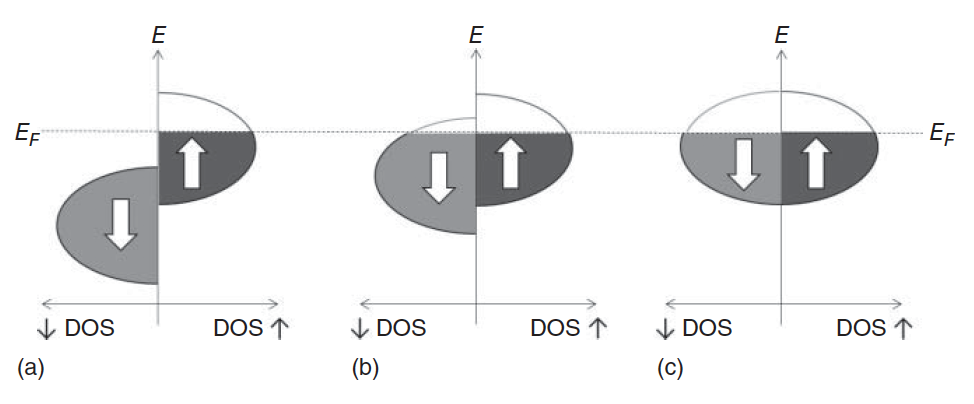
\includegraphics[width=130mm]{fig/review/dos.png}
	\caption[Schematic densities of states (DOSs) for ferromagnetism.]{Schematic densities of states (DOSs) for FM: (a) strong FM, (b) weak FM, and (c) PM.}
\label{fig:dos}
\end{figure}

Meanwhile, there is another type of magnets that possess magnetization
microscopically, but have no macroscopic magnetization due to the cancelation
of antiparallel spins of neighboring pairs – this is known as AFM phase.
A magnet that exhibits no macroscopic magnetization at high temperature (when $H = 0$) is known as the PM phase, in which the magnetic moment induced by the applied H-field is rather weak.
 Figure~\ref{fig:temp_mag} shows the relationship
between magnetization and temperature of a FM, where one can see
that the magnetization starts decreasing close to $T_C$, and when $T >T_C$, magnetic
moments align randomly resulting in zero macroscopic magnetization.
\begin{figure}[H]
	\centering
	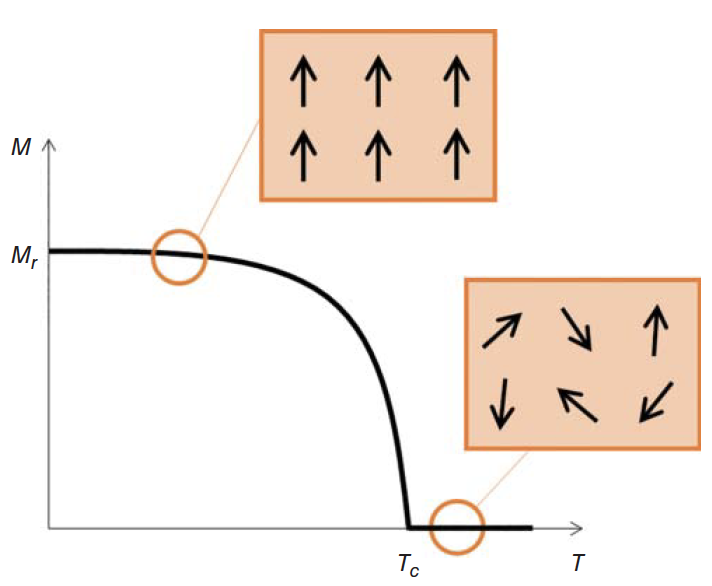
\includegraphics[width=100mm]{fig/review/temp_mag.png}
	\caption[Illustration of magnetization versus temperature.]{Illustration of magnetization versus temperature.}
\label{fig:temp_mag}
\end{figure}

Any atoms or ions with existing unpaired electrons exhibit ferromagnetism such as Fe, Co, and Ni. Magnetization can exist, even very weak, in non-FM materials such as graphene as long as their defects or edge structures induce dangling bonds with unpaired electrons \cite{Ma:2012aa, Liu:2013aa}. However, those FM materials with known practical application potentials are usually compounds containing Fe, Co, or Ni.

\section{Magnetic anisotropy}
Magnetic anisotropy is defined as the directional dependence of the magnetic
properties for materials. Specifically, the preferential direction for its magnetic moment in the absence of an applied magnetic field. Strong easy-axis anisotropy is a prerequisite for hard magnetism, while near-zero anisotropy is desirable for soft magnets.
Generally, the tendency for magnetization to lie along an easy axis is represented by the energy
density term:
\begin{equation}
E_a = K_1 \sin^2 \theta
\end{equation}

where $\theta$ is the angle between the magnetic field and the anisotropy axis, and $K_1$ is the
anisotropy constant, which ranges from $~1 kJ/m^3$ to more than $20 MJ/m^3$.  There are
several sources of magnetic anisotropy:
\begin{itemize}
\item Magnetocrystalline anisotropy: intrinsic property due mainly to spin-orbit coupling;
\item Shape anisotropy: induced by the nonspherical shape of the grains; 
\item Stress anisotropy: created by applied mechanical stress due to the existence of magnetostriction, which could alter the domain structure;
\item Exchange anisotropy: occurs when the interaction between antiferromagnet and a ferromagnet occurs at their interface;
\item Anisotropy induced by grain alignment and stress through magnetic
annealing, irradiation, and plastic deformation.

\end{itemize}

\section{Magnetocrystalline anisotropy}
The magnetocrystalline anisotropy primarily arises from spin-orbit coupling.
When an external field tries to reorient the spin of an electron, the orbit of that electron
also tends to be reoriented. But the orbit is strongly coupled to the lattice and therefore
resists the attempt to rotate the spin axis. The energy required to rotate the spin system of
a domain away from the easy direction, anisotropy energy, is the energy required to
overcome the spin-orbit coupling. The strength of the magnetocrystalline anisotropy in
any particular crystal is measured by the magnitude of the anisotropy constant $K_1$, $K_2$, etc.

The magnitude of the magnetocrystalline anisotropy generally decreases with
temperature more rapidly than the magnetization vanishes at the Curie temperature. Since
the anisotropy contributes strongly to the coercive field, it has a great influence on
industrial uses of FM materials. Materials with high magnetic anisotropy
usually have high coercivity; that is they are hard to demagnetize.
The high anisotropy of REEs metals is mainly responsible for the strength of widely used magnets containing them.


\section{Domain and Domain Walls}
In FM, materials, exchange, and dipolar couplings are competing.
The equality between both interactions leads to a state in which the local macroscopic magnetization is extremely small. Still, an almost parallel alignment of the moments is preserved at short distances.
In the absence of magnetocrystalline anisotropy, a gradual rotation of the moments takes place.
Overall, the material splits into a number of isolated zones, called magnetic domains.
Within each domain, the moments are parallel as required by coupling, the magnetization is directed along a precise so-called easy direction, as required by anisotropy. From one zone to another, the direction of magnetization changes so that the total magnetization disappears.
Between two neighboring domains, a gradual rotation of the moments takes place which defines a Bloch wall. A Bloch wall has a special parameter characteristic thickness, $\delta$, for which its value of energy per unit area, $\gamma$, is minimum. $\delta$ and $\gamma$ are given by :
\begin{align}
\delta = \pi \sqrt{A/K} \\
\gamma = 4 \sqrt{AK}
\end{align}

here $A$, the exchange constant expressed in $J/m$, characterises the strength of the exchange coupling and $K$ is the anisotropy constant expressed in $J/m^3$.
Most typically $\delta$ varies from 50 nm
in the $3d$ metals to 3 nm in high-anisotropy compounds (\ce{SmCo5}, \ce{Nd_2Fe_{14}B}).

\begin{table}[H]
\caption[Domain wall thickness]{Domain wall thickness}
\centering

\begin{tabular}{|l|c|}

\hline 
Magnetic material & Domain wall width (nm) \\ 
\hline 
Co & 14 \\ 
\ce{Nd_2Fe_{14}B} & 3.9 \\ 
\ce{Sm_2Fe_{17}N_3} & 3.6 \\ 
\ce{Sm_2Co_{17}} & 8.6 \\ 
FePd & 11.4 \\ 
\hline 
\end{tabular} 

\end{table}

In the general case, splitting of a FM material into domains separated by walls occurs spontaneously.
In a homogeneous material, the wall energy does not depend on the wall position.
 Under an applied external field $H$, the initial magnetization variation is to minimize the Zeeman energy and the dipolar energy. In a system of cubic symmetry, the susceptibility is equal to the inverse of the demagnetizing field slope; it is defined by the sample shape and not connected to the intrinsic material properties.
During this process, the magnetization variation occurs by growing the domains aligned by the applied field at the expense of others. The material is in the single domain state at a larger field, and magnetization variation occurs by moment rotation.


FM materials also exhibit domain structure where each domain has its own magnetization direction that can be switched by external magnetic field.
There are easy axes in FM materials that are the directions magnetic
moments should follow. For example, for a cubic structured FM material such as
Fe, the $\langle 100 \rangle$ directions are usually the easy axes, while for a hexagonal-structured FM material such as Co, the $\langle 0001\rangle$ are the easy axes. Due to this difference, in a cubic structure, both $90 ^\circ$ and $180^\circ$ magnetic domains can be formed (Figure~\ref{fig:domain_structure}a), while in a hexagonal structured FM material, the domains are usually aligned with an angle of $180 ^\circ $ (Figure~\ref{fig:domain_structure}b).

\begin{figure}[H]
\centering
\captionsetup{justification=centering,margin=2cm}
	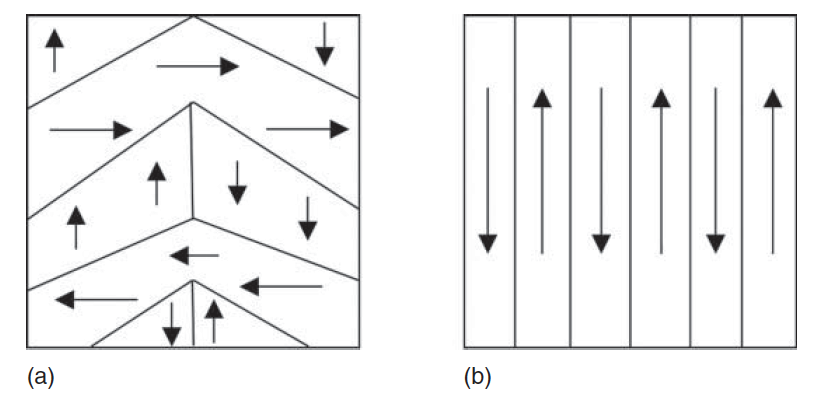
\includegraphics[width=110mm]{fig/review/domain_structure.png}
	\caption[Domain structures in cubic and FM materials.]{Domain structures in cubic (a) and hexagonal (b) structured FM materials.}
\label{fig:domain_structure}
\end{figure}

The easy axes of cubic-structured Ni are $\langle 111 \rangle$, so it can form $180 ^\circ$, $71 ^\circ$, and $109 ^\circ$ magnetic domains; these are possible angles between all $\langle 111 \rangle$ easy axes. The magnetization switching can be realized by not only external magnetic field but also mechanical stress.

FM domain wall is only one to a few atomic layers. Figure~\ref{fig:wall_structure}a illustrates the $180  ^\circ$ domain wall structure in FM materials, where the more common one is the Bloch wall, but in thinner films a Néel wall is often favored Figure \ref{fig:wall_structure}b. By contrast, Figure \ref{fig:wall_structure}c demonstrates a narrow domain wall (Ising type) structure usually as the case of a ferroelectric domain structure.

\begin{figure}[H]
\centering
\captionsetup{justification=centering,margin=2cm}
	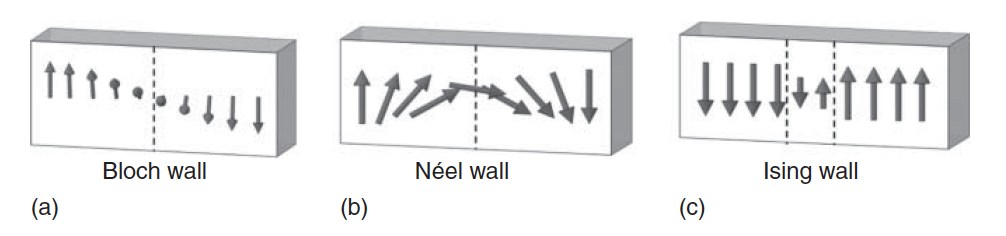
\includegraphics[width=150mm]{fig/review/wall_structure.png}
	\caption[Domain wall structures.]{Domain wall structures of (a) Bloch-type FM domain walls, (b) Néel-type FM domain walls, and (c) Ising-type ferroelectric domain walls.}
\label{fig:wall_structure}
\end{figure}

\section{T-symmetry}
Generally T-symmetry or Time Reversal symmetry is the symmetry of physical laws under a time reversal transformation $( \tau )$.
\begin{equation}
\tau : t \rightarrow -t
\end{equation}

The origin of ferromagnetism (FM) is time reversal symmetry breaking due to the existence of unpaired spin of electrons and the associated current \cite{eerenstein2006multiferroic}. 
This statement
can be understood by considering that if time is reversed, the spin or current
flow direction will thus be reversed and this results in magnetization direction
reversion, i.e. time reversal symmetry breaking.

\begin{equation}
\tau : \mu = - \mu
\end{equation}

In other words as it is illustrated on Figure \ref{fig:time_reverse} the local magnetic moment \textbf{m} may be represented classically by a charge that dynamically traces an orbit, as indicated by the arrowheads. A spatial inversion produces no change, but time reversal switches the orbit and thus \textbf{m}.

\begin{figure}[H]
	\centering
	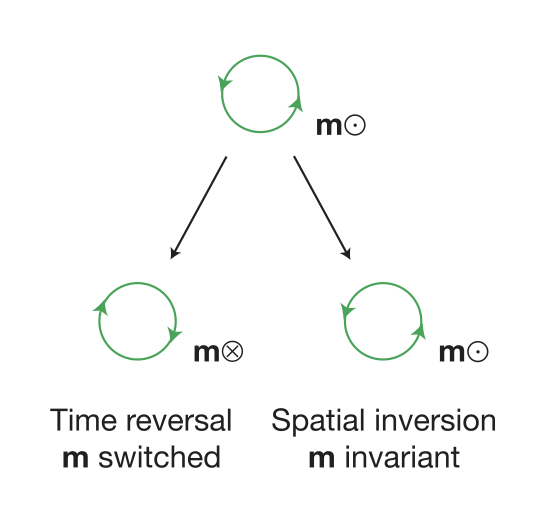
\includegraphics{fig/review/time_reverse.png}
	\caption[Illustration of time reversion symmetry breaking]{Illustration of time reversion symmetry breaking \cite{eerenstein2006multiferroic}}
\label{fig:time_reverse}
\end{figure}

Thus, magnetic ordering always breaks at least one symmetry of the crystal, the invariance under time inversion. Invariance under rotations around axes not coinciding with the ordered moments also disappears. This symmetry braking is not related to asymmetries in the spin Hamiltonian.
Spin Hamiltonians are constructed to describe the behaviour of the degrees of freedom of atoms or ions occupying lattice sites.
Therefore, they have the full symmetry of the lattice.


\section{Magnetic models}\label{section: Magnetic models}

\subsection{Ising model}
Ising or 1/2-spin model is known as one of the most famous and simplest theoretical representations of magnetic systems. Despite this fact, this model has proven to be convenient for the descriptions of rather complicated interactions giving quite accurate results and being pretty useful as a test case for new approximations in systems of interacting particles even not related to magnetism.  For instance, presently, it is applied to study liquids freezing and evaporation, ordered-disordered transformation in alloys, the behavior of glassy substances, and even active form of protein molecules.

In the framework of original model, every discrete spin of the lattice is presented as +1 or -1.
For the case of a one-dimension, it is a chain of spins, every of which has only nearest-neighbor interaction. Ising himself rigorously solved this model in 1924 in his PhD work.

In two dimensional case, this model is a square lattice with an equal number of spins in two directions. Each spin interacts with two nearest neighbors in both lateral axes (4 in total). This model was intensively studied theoretically by various methods like Green functions, mean-field theory, high and low-temperature series expansion, transfer matrixes but so far was solved only for the case of an absent external magnetic field.  Cases of two-dimensional models with applied external field or simplest examples of the three-dimensional magnetic model remain unsolved.

The most common representation of Ising model for ferromagnetic material in applied external field $H$ given by following Hamiltonian:

\begin{equation}
{\cal H}_{Ising} = -\sum \limits_{i, j} J_{ij} S_i S_j - H \sum \limits_{i} S_i
\end{equation}

Here $J_{ij}$ is exchange interaction between spins in different lattice sites $S_i$ and $S_j$ respectively.

In a framework of this model positive value of nearest-neighbors exchange coupling $J_{ij}>0$ represents a ferromagnetic system, negative $J_{ij}<0$ antiferromagnetic, and zero $J_{ij}=0$ nonmagnetic as spins don't interact with each other.

Typically this model might be additionally modified to represent more complex systems with an addition of coupling with next nearest-neighbors or dipole interaction.

\subsection{Heisenberg model}
More complex Heisenberg spin model related to prototypical Ising theory has a form of following Hamiltonian:
\begin{equation}
{\cal H}_{Heisenberg} = -\sum \limits_{i, j} J_{ij} S_i S_j - H \sum \limits_{i} S_i - K\sum \limits_{i} (S_i^z)^2
\end{equation}

In this case variable $S_i$ related to spin already represents 3D vectors with $|S_i| = S$. While $K$ denotes a magnetocrystalline anisotropy of a single ion in the system.

In the case of extreme anisotropy,  we can find the Hamiltonians which define two important models.

In a case of extremely high anisotropy when the limit of infinite single-ion anisotropy $K\rightarrow~\infty$. All the magnetic moments tend to align to the point in one direction and Heisenberg model reduces to already known to us, Ising model.

On the opposite case when $K \rightarrow -\infty$.  All the spins tend to lie in one plane and Heisenberg model reduces to XY model. 

Hence Ising model represents the spin variety in a single dimension, XY model allows spin rotation in 2D case, and the Heisenberg model denotes spin variety in tree dimensions. Therefore varying value of anisotropy in a Heisenberg spin model we may allow system to approach behavior typical for XY or Ising model without any contradictions.

As the Ising and XY models exclude some components of the spin vectors, the entities they describe can be looked upon as one- and two-dimensional moments, respectively.
However, this does not automatically make them low-dimensional models. The dimensionality is determined by the meaning of the indices $i$ and $j$. Those indicate sites in a lattice of well defined dimension.
Thus one can study three-dimensional Ising models or one-dimensional XY models; there is also no contradiction in terms here.


\subsection{Phase Transitions }
In thermodynamics phase transition defined as a physical process at which system order parameter undergoes changes from zero in one state to non-zero in another. The behavior of order parameter as a function of some variables like temperature determine a certain point in which systems transits from one phase to another.

The first and second types of phase transition are distinguished by the type of change in the order parameter. In the first type of transition, the order parameter will intermittently change from zero to a certain value, while the system can be in both states simultaneously. In the second type, also known as a continuous phase transition, the order parameter will gradually change, reaching a certain value.

The order parameter for ferromagnetic systems is the magnetization which is continuously falls to zero while the system reaches a its critical temperature $(T_C)$ also known as Curie temperature.

Continuous phase transition under consideration is also might be characterized by a series of quantities called critical exponents, denoting their relations with a critical point. In magnetic systems these exponents difend for zero field specific heat, magnetization and susceptibility by following equation:

\begin{equation}
C \propto |T-T_C|^{-\alpha},
\end{equation}

which characterize the behavior of a ferromagnetic system specific heat $C$ near the Curie point. This exponent are interesting because of universality: systems that appear different but have a few essential properties in common possess the same critical exponent.
A universality class comprises systems which exhibit this behavior, e.g. certain ferromagnetic systems and the liquid-gas phase transition for fluids. The thermodynamic properties of the system would seem to depend only on the few parameters, such as dimensionality and symmetry

\section{Monte Carlo Simulations}\label{section: Monte Carlo method}

\subsection{Monte Carlo method}
Monte Carlo method have proven effective in a wide variety of areas. For example, today, this method is used to predict financial markets and risk analysis, modeling biological processes, studying black holes, and solving differential equations, artificial intelligence, chemistry, and so on.  Despite the complexity of the stated problems, this method is based on fairly simple and intuitive principles, which explains its high popularity.

The method can be summarized as follows: a set of random values ​​is generated for a target random variable, and then the required values ​​are calculated on its basis. The modern version of the method was formed in the framework of the Manhattan Project, where it was used to simulate the distances that neutrons can travel in various materials. The idea of ​​modeling based on the generation of a set of random values ​​has already existed for some time before, but it was specially developed with the creation of the atomic bomb and then spread to many other luckily more peaceful areas of knowledge.

The big advantage of Monte Carlo method is that it allows for the element of randomness and complexity of the real world to be taken into account in the model. In addition, the method is robust concerning changes in various parameters, such as the distribution of a random variable. 

\subsection{Monte Carlo in Statistical Mechanics}

From the viewpoint of statistical mechanics, Monte Carlo method allows computing the internal energy of the system based on its particle states. Hence from the Maxwell-Boltzman statistics, the probability of the system to be in a specific state $a$ can be written as follows:

\begin{equation}
p_a = \frac{1}{Z}e^{-\beta E_a}.
\end{equation}


Here $\beta = \frac{1}{kT}$, $T$  -temperature, $E_a$ - internal system energy,  Z - partition function defined as:

\begin{equation}
Z = \sum \limits_{a} e^{-\beta E_a}.
\end{equation}

In a specific case of ferromagnetic system study the expectation value (avarage over different system states) of its magnetization might be written as:

\begin{equation}
\langle m \rangle = \frac{1}{Z}\sum \limits_{a}m_a e^{-\beta E_a}.
\end{equation}

In the same fashion, we can also write an equation for the energy of the system.

\begin{equation}
\langle E \rangle = \frac{1}{Z}\sum \limits_{a}E_a e^{-\beta E_a}.
\end{equation}

\subsection{Metropolis algorithm}
Despite the apparent simplicity of the Ising spin model described in section  \ref{section: Magnetic models} in practice, it is often difficult to simulate numerically for the systems with a high number of states.  For instance considering Ising model for the system with $N$ sites of the lattice and 2 possible individual spin values $S\in \{-1, +1 \}$ its ends up with $\{-1, +1 \}^N$ or simply $2^N$ possible states. Shown level of complexity motivates the application of Monte Carlo techniques in the simulation in a framework of Ising model.

Used in this case Hamiltonian has a slightly simplified form: 

\begin{equation}
{\cal H} (a) = -J \sum \limits_{i, j}  S_i S_j - H \sum \limits_{i} S_i
\end{equation}

Which might be simplified even more assuming zero contribution of the applied external field $H$. Such simplification is justified since many questions described by the considered model might be solved in the absence of an external field.  Hereby the following equation denotes the energy of the systems in state $a$.

\begin{equation}
{\cal H} (a) = -J \sum \limits_{i, j}  S_i S_j
\end{equation}

Given simplified version of Hamiltonian allows calculating several properties of magnetic materials such as specific heat or magnetization at a given temperature.

The Metropolis-Hastings algorithm is the most frequently used algorithm for the Ising model simulations.  As an initial stage algorithm chooses the probabilities $p(a,  b)$ which denotes the possibility of the algorithm to choose state $b$ when the system is in a state $a$.
It then uses acceptance probabilities $A(a, b)$ so that demand of detailed balance is satisfied.  If the new state $b$ is accepted, then we move to that state and repeat with selecting a new state and deciding to accept it. If $b$ is not accepted then we stay in $a$. This process is repeated until some stopping criterion is met, which for the Ising model is often when the lattice becomes ferromagnetic. 

Given alghoritm follows the concept of single-spin-flip dynamics, which states that in each transition, we will only change one of the spin sites on the lattice. Furthermore, by using single- spin-flip dynamics, one can get from any state to any other state by flipping each site that differs between the two states one at a time.

The derivation of the Metropolis algorithm follows from a few simple steps. From state a, there are $N$ possible states that can be reached after one flip to create different states. The probability to create a specific state $b$ from $a$ is thus $g(a, b) = \frac{1}{N}$, as they
are all equally favored; the probability of creating state $a$ from $b$ is also the same. The condition of detailed balance, which follows from,  can then be stated as:

\begin{equation}
\frac{P(a, b)}{P(b,a)} = \frac{A(a, b)g(a,b)}{P(b,a)g(b,a)}=\frac{A(a,b)}{A(b,a)} = \frac{\frac{1}{Z} e^{\beta E_b}}{\frac{1}{Z} e^{\beta E_a}}=e^{-\beta(E_b - E_a)}
\end{equation}

The choice of acceptance ratio can be made in almost any fashion, so long as this equation is obeyed; however, a low acceptance ratio would lead to many wasted calculations,
and as such a large acceptance ratio is therefore generally more efficient. In general the acceptance probabilities chosed to satisfy:

\begin{equation}
\frac{A(a,b)}{A(b,a)} = e^{-\beta(E_b - E_a)}
\end{equation}

if $E_b > E_a$, then $A(b,a) > A(a,b)$. Metropolis sets the larger of $A(a, b)$ or $A(b, a)$ to be 1. By this reasoning the acceptance algorithm is:

\begin{equation}
A(a,b) = 
  \left\{
    \begin{aligned}
      & e^{-\beta(E_b - E_a)}, \ if \ E_b - E_a > 0 \\
      & 1, \ else
    \end{aligned}
  \right.
\end{equation}

As a summary to the usage of the Metropolis algorithm in Monte Carlo simulations,
the following steps are done for one application of the algorithm:
\begin{enumerate}
\item Calculate the energy of the system.
\item Pick a random spin on the lattice.
\item Calculate the energy if the spin is flipped and $\Delta E = e^{-\beta(E_b - E_a)}$, the difference in energy between this energy and the previous one.
\item If $\Delta E < 0$,the spin is flipped. Otherwise, the next step is followed.
\item Calculate the Boltzmann weight $w = e^{-\beta(E_b - E_a)}$.
\item Generate a random number $0 \leq r < 1$.
\item If $r < w$, flip the spin. If not, no change is made.
\end{enumerate}


